\documentclass[9pt,journal]{IEEEtran}

%\usepackage[brazil]{babel}
%\usepackage[latin1]{inputenc}
%\usepackage{ucs}
%\usepackage[utf8x]{inputenc}
%\usepackage[T1]{fontenc}
\usepackage[utf8]{inputenc}
\usepackage{graphicx}


\begin{document}

	%--------------------------------------------------------
	% Capa e Folha de Rosto
	%--------------------------------------------------------
	\title{Route Generator to Indoor Environments Monitoring Using Mobile Robots}
	\author{Heitor~Luis~Polidoro, Dr.~Denis~Fernando~Wolf}
%	\supervisor{Prof. Dr. Denis Fernando Wolf}
	\date{São Carlos / SP\\Junho de 2009}
%	\concarea{Robótica Móvel, Monitoramento, Navegação.}
	\maketitle
	%--------------------------------------------------------

	\begin{abstract}
One of the main challenges in the area of mobile robots is the development of autonomous systems that are able to interact with the environment, and learn to take correct decisions for their tasks are carried out successfully. The development of these intelligent and autonomous systems is an area of multidisciplinary research promising that involves: artificial intelligence, machine learning, statistical estimation, embedded systems and other areas of computer science.
	
The monitoring of environments using mobile robots is a problem that has received great attention from the scientific community. Given a representation of the environment (map) and a list of priorities, the robot must decide which way to follow to covered the environment in the most efficient way possible. There are several practical applications for this type of algorithm, among them there is the development of intelligent safety systems.
	\end{abstract}

	\section{Introduction}

The robotics consist in a multidisciplinary research area, involving mechanic, electric and computer engineering and human areas such as psychology and animal behaviors study.

Initially, the robots were used in industrial automation, but with the technological developments the robots have been used in other areas such as: medical, precision, hazardous environments, entertainment, household services, etc.. In this context came the search for the development of autonomous mobile robots that are capable of acting in real environments and react to unfamiliar situations in an intelligent manner.

The mobile robot, besides being an area of great scientific potential, technology companies are increasingly investing in products. Such as the development of robots that perform housework independently, including the Roomba, a vacuum cleaner robot of IRobot \cite{IRobot}, the Friendly Robotics' lawn-mower robot, Robomow \cite{FriendlyRobotics}, and the PatrolBot of MobileRobots \cite{MobileRobotsPatrolBot} that can be set for security purposes.

This paper propose a strategy to monitor indoor environments, where, usually, in those environments, there are critical areas with different priorities to be visited. The strategy must find the best path to monitor each environment according to the priority of each critical area. As the environment monitoring task has no determined duration, the results in a loop, that the robot should keep following to visit the entire environment. There are some strategies to find paths, such as Vehicle Routing Problem (VRP) and the Traveler Salesmen Problem \cite{Arenales2007}, but both are based in visiting each node once per loop, the results for the problem exposed in this paper might have loops that, one or more nodes, or critical area, are visited more then once per loop according to each priority. For this kind of problem nothing was found in the literature.


	\section{Indoor Environment Monitoring}
	
To do an environment monitoring, first is necessary divide this environment in interest areas, and assign, for each area, a priority relative to the importance that area represents. So, the robot must visit these areas respecting their priorities. The Picutre \ref{fig:planta} shows an example of an divided environment, and the Table \ref{tab:exemplo} show an example of priorities.

\begin{figure}%
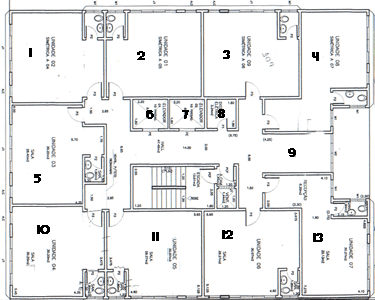
\includegraphics[width=\columnwidth]{imagens/planta_numerada.png}%
\caption{An example of an environment divided in critical areas}%
\label{fig:planta}%
\end{figure}

\begin{table}%
\centering
\caption{Example of priorities}
\begin{tabular}{|l|l|l|l|l|l|l|l|l|l|l|l|l|l|}
\hline
Room & 1 & 2 & 3 & 4 & 5 & 6 & 7 & 8 & 9 & 10 & 11 & 12 & 13 \\ 
\hline
Priority & 5 & 5 & 2 & 1 & 3 & 2 & 1 & 2 & 1 & 4 & 4 & 2 & 3 \\ 
\hline
\end{tabular}
\label{tab:exemplo}
\end{table}

Each room has an Urgency Factor which is derived by multiplying the room priority by the time since the last visit, as show in the equation \ref{eq:urgencia}.

\begin{eqnarray}
U_i= P_i \times t_i
\label{eq:urgencia}
\end{eqnarray}









	\bibliographystyle{plain}
	\bibliography{bibliografia}

\end{document}
